\documentclass[12pt]{article}
\usepackage{fullpage}
\usepackage[utf8]{inputenc}
\usepackage{pict2e}
\usepackage{amsmath}
\usepackage{enumitem}
\usepackage{eurosym}
\usepackage{pict2e}
\usepackage{mathtools}
\usepackage{amssymb, amsfonts, latexsym, cancel}
\setlength{\parskip}{0.3cm}
\usepackage{graphicx}
\usepackage{fontenc}
\usepackage{slashbox}
\usepackage{setspace}
\usepackage{gensymb}
\usepackage{accents}
\usepackage{adjustbox}
\setstretch{1.5}
\usepackage{bold-extra}
\usepackage[document]{ragged2e}
\usepackage{subcaption}
\usepackage{tcolorbox}
\usepackage{xcolor, colortbl}
\usepackage{wrapfig}
\usepackage{empheq}
\usepackage{array}
\usepackage{parskip}
\usepackage{arydshln}
\graphicspath{ {images/} }
\renewcommand*\contentsname{\color{black}Índice} 
\usepackage{array, multirow, multicol}
\definecolor{lightblue}{HTML}{007AFF}
\usepackage{color}
\usepackage{etoolbox}
\usepackage{listings}
\usepackage{mdframed}
\setlength{\parindent}{0pt}
\usepackage{underscore}
\usepackage{hyperref}
\usepackage{tikz}
\usepackage{tikz-cd}
\usetikzlibrary{shapes, positioning, patterns}
\usepackage{tikz-qtree}
\usepackage{biblatex}
\usepackage{pdfpages}
\usepackage{pgfplots}
\usepackage{pgfkeys}
\addbibresource{biblatex-examples.bib}
\usepackage[a4paper, left=1.5cm, right=1.5cm, top=1cm,
bottom=1.5cm]{geometry}
\everymath{\displaystyle}
\usetikzlibrary{decorations.pathreplacing}
\usepackage{titlesec}
\usepackage{titletoc}
\usepackage{tikz-3dplot}
\usetikzlibrary{decorations.pathreplacing}
\newcommand{\Ej}{\textcolor{lightblue}{\underline{Ejemplo}}}
\setlength{\fboxrule}{1.5pt}
\renewcommand{\arraystretch}{1.35}
\setlength{\arraycolsep}{0.3cm}

% Configura el formato de las secciones utilizando titlesec
\titleformat{\section}
{\color{red}\normalfont\LARGE\bfseries}
{Tema \thesection:}
{10 pt}
{}

% Ajusta el formato de las entradas de la tabla de contenidos
\addtocontents{toc}{\protect\setcounter{tocdepth}{4}}
\addtocontents{toc}{\color{black}}

\titleformat{\subsection}
{\normalfont\Large\bfseries\color{red}}{\thesubsection)}{1em}{\color{lightblue}}

\titleformat{\subsubsection}
{\normalfont\large\bfseries\color{red}}{\thesubsubsection)}{1em}{\color{lightblue}}

\newcommand{\bboxed}[1]{\fcolorbox{lightblue}{lightblue!10}{$#1$}}

\DeclareMathOperator{\N}{\mathbb{N}}
\DeclareMathOperator{\Z}{\mathbb{Z}}
\DeclareMathOperator{\R}{\mathbb{R}}
\DeclareMathOperator{\Q}{\mathbb{Q}}
\DeclareMathOperator{\K}{\mathbb{K}}
\DeclareMathOperator{\im}{\imath}
\DeclareMathOperator{\jm}{\jmath}
\DeclareMathOperator{\col}{\mathrm{Col}}
\DeclareMathOperator{\fil}{\mathrm{Fil}}
\DeclareMathOperator{\rg}{\mathrm{rg}}
\DeclareMathOperator{\nuc}{\mathrm{nuc}}
\DeclareMathOperator{\dimf}{\mathrm{dimFil}}
\DeclareMathOperator{\dimc}{\mathrm{dimCol}}
\DeclareMathOperator{\dimn}{\mathrm{dimnuc}}
\DeclareMathOperator{\dimr}{\mathrm{dimrg}}

\newcommand{\bu}[1]{\textcolor{lightblue}{\underline{#1}}}
\newcommand{\lb}[1]{\textcolor{lightblue}{#1}}
\newcommand{\db}[1]{\textcolor{blue}{#1}}
\newcommand{\rc}[1]{\textcolor{red}{#1}}
\newcommand{\tr}{^\intercal}

\renewcommand{\CancelColor}{\color{lightblue}}

\newcommand{\dx}{\:\mathrm{d}x}
\newcommand{\dt}{\:\mathrm{d}t}
\newcommand{\dy}{\:\mathrm{d}y}
\newcommand{\dz}{\:\mathrm{d}z}
\newcommand{\dth}{\:\mathrm{d}\theta}
\newcommand{\dr}{\:\mathrm{d}\rho}
\newcommand{\du}{\:\mathrm{d}u}
\newcommand{\dv}{\:\mathrm{d}v}
\newcommand{\tozero}[1]{\cancelto{0}{#1}}
\newcommand{\lbb}[2]{\textcolor{lightblue}{\underbracket[1pt]{\textcolor{black}{#1}}_{#2}}}
\newcommand{\dbb}[2]{\textcolor{blue}{\underbracket[1pt]{\textcolor{black}{#1}}_{#2}}}
\title{Cálculo 2\quad 17/01/2024}

\begin{document}
  \begin{enumerate}[label=\arabic*)]
    \item \lb{Contestar razonadamente las siguientes preguntas:}
      \begin{enumerate}[label=\color{red}\alph*)]
        \item \db{Definir con precisión qué se entiende por el plano tangente de una función $z=f(x,y)$ en un punto  $(x_0,y_0)$ de su dominio. Como aplicación, obtener el valor de $\alpha$ de forma que la función $f(x,y)=\alpha x^2+y^2-2x-1$ tenga a $2x-2y+z=0$ como plano tangente en el punto  $(1,1)$.}

          El plano tangen de una función $z=f(x,y)$ en un punto  $(x_0,y_0)$ del dominio se define como el plano que mejor aproxima a la superficie $z=f(x,y)$ en ese punto. Este plano está dado por la ecuación:  \[
          z-f(x_0,y_0)=\frac{\partial f}{\partial x}(x_0,y_0)(x-x_0)+\frac{\partial f}{\partial y} (x_0,y_0)(y-0). 
          \] 

          Queremos que el plano tangente de la función $f(x,y)=\alpha x^2+y^2-2x-1$ en el punto  $(1,1)$ sea:  \[
          2x-2y+z=0.
          \] 
          Las derivadas parciales de $f(x,y)$ son:  \[
          \begin{array}{c}
            \frac{\partial f}{\partial x} (x,y)=\frac{\partial }{\partial x} (\alpha x^2+y^2-2x-1)=2\alpha x-2\\
            \frac{\partial f}{\partial y} (x,y)=\frac{\partial }{\partial y} (\alpha x^2+y^2-2x-1)=2y
          \end{array}
          \] 
          En $(1,1)$ evaluamos:  \[
          f(1,1)=\alpha\cdot 1^2+1^2-2\cdot 1-1=\alpha+1-2-1=\alpha-2\\
          \frac{\partial f}{\partial x} (1,1)=2\alpha-2\\
          \frac{\partial f}{\partial y} (1,1)=2
          \] 
          La ecuación del plano tangente en $(1,1,f(1,1))$ es:  \[
            \begin{aligned} 
              z-f(1,1)&=\frac{\partial f}{\partial x} (1,1)(x-1)+\frac{\partial f}{\partial y} (1,1)(y-1)\\
              z-\alpha+2&=(2\alpha-2)x - (2\alpha-2) +2y-2\\
              z&=(2\alpha-2)x+2y-2\alpha+2-2+\alpha-2\\
              z&=(2\alpha-2)x+2y-\alpha-2\\
              z&= 2\alpha x-2x+2y-\alpha-2 \\
            \end{aligned}
          \] 
          El plano tangente debe coincidir con $2x-2y+z=0$, que puede reescribirse como:  \[
          z=-2x+2y
          \] 
          Companado términos:

          \[
            (2\alpha-2)x=-2x\longrightarrow 2\alpha-2=-2\longrightarrow 2\alpha=0\longrightarrow \alpha=0.
          \]
        El valor de $\alpha$ para que el plano tangente sea $2x-2y+z=0$ en el punto  $(1,1)$ es:  \[\bboxed{\alpha=0}\] 
        \item \db{Determinar si el conjunto \[
        B=\{(x,y)\in \R^2:y^2>1\}
        \]es cerrado o abierto $\R^2$ con la norma euclídea y, al mismo tiempo, calcular el interior de clausura, la frontera y los puntos de acumulación.}

        El conjunto dado es: \[
        B=\{(x,y)\in \R^2:y^2>1\}. 
        \] 
        Esto representa los puntos del plano $\R^2$ cuya coordenada $y$ satisface  $y>1$ o  $y<-1$.

        El conjunto $B$ es abierto porque para todo punto $\mathbf{x}\in B$ existe un número real positivo $\mathcal{E}>0$ de manera que la bola abierta $A(\mathbf{x},\mathcal{E})$ está contenida completamente en $B$.
        \begin{center}
          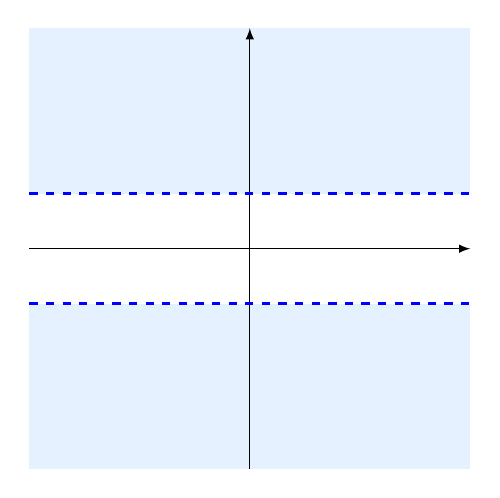
\begin{tikzpicture}[scale=0.7]
          \fill[color=lightblue!20, opacity=0.5] (-4,1) rectangle (4,4);
          \fill[color=lightblue!20, opacity=0.5] (-4,-1) rectangle (4,-4);
          \draw[-latex] (0,-4) -- (0,4);
          \draw[dashed, blue, line width=1.2] (-4,1) -- (4,1);
          \draw[dashed, blue, line width=1.2] (-4,-1) -- (4,-1);
          \draw[-latex] (-4,0) -- (4,0);
        \end{tikzpicture}
      \end{center}
      El interior del conjunto $B$ es el conjunto de puntos que tienen un vencidad completamente contenida en  $B$. En este caso, el interior es todo el conjunto  $B$ ya que todos los puntos en  $B$ cumplen  $y^2>1$ y tienen una vencidad contenida en $B$
      \item \db{Demostrar que para cualquier función $f:\R^3\to \R$ de clase $C^2$ se cumple que $\mathrm{rot} (\mathrm{grad} f)=\nabla \times (\nabla f)=0$.} 

        Sea $f:\R^3\to \R$ una función escalar de clase  $C^2$, es decir, sus derivadas parciales de primer y segundo orden son continuas. Queremos demostrar que el rotacional del gradiente de $f$es siempre cero:  \[
        \nabla \times (\nabla f)=0
        \] 
        El gradiente de $f$ es:  \[
        \nabla f=\left( \frac{\partial f}{\partial x} ,\frac{\partial f}{\partial y} ,\frac{\partial f}{\partial z}  \right) .
        \] 
        El rotacional de $\nabla f$ es: \[
        \nabla \times (\nabla f)=\begin{vmatrix} 
          \mathbf{i}  & \mathbf{j} & \mathbf{k} \\
          \frac{\partial }{\partial x} & \frac{\partial }{\partial y} & \frac{\partial }{\partial z}\\
          \frac{\partial f}{\partial x} & \frac{\partial f}{\partial y} & \frac{\partial f}{\partial z} \\
        \end{vmatrix}=\mathbf{i} \left( \frac{\partial }{\partial y} \left( \frac{\partial f}{\partial z} \right) -\frac{\partial }{\partial z} \left( \frac{\partial f}{\partial y}  \right)  \right) -\mathbf{j} \left( \frac{\partial }{\partial z} \left( \frac{\partial f}{\partial x}  \right) -\frac{\partial }{\partial x} \left( \frac{\partial f}{\partial z}  \right)  \right) + \mathbf{k} \left( \frac{\partial }{\partial x} \left( \frac{\partial f}{\partial y}  \right) -\frac{\partial }{\partial y} \left( \frac{\partial f}{\partial x}  \right)  \right)
        \] 
        Como $f$ es de clase  $C^2$, por el \textbf{teorema de Schwarz} las derivadas parciales mixtas son iguales y por eso: \[
        \mathbf{i} \left( \frac{\partial^2 f}{\partial z \partial y} -\frac{\partial^2 f}{\partial y \partial z}  \right) -\mathbf{j} \left( \frac{\partial^2 f}{\partial x \partial z} -\frac{\partial^2 f}{\partial z \partial x}  \right) + \mathbf{k} \left( \frac{\partial^2 f}{\partial x \partial y} - \frac{\partial^2 f}{\partial y \partial z}  \right) =(0,0,0)
        \]  
        Dado que todas las componentes del rotacional son cero, tenemos: \[
        \nabla \times (\nabla f)=0.
        \] 
      \end{enumerate}
    \item \lb{Consideramos la función \[
    f(x,y)=\begin{cases}
      \dfrac{y^3+k(x^2+y^2)}{x^2+y^2} & \text{si }(x,y)\neq (0,0)\\
      \sqrt{2} & \text{si }(x,y) =(0,0)
    \end{cases}
    \] donde $k$ es un número real. Encontrar el valor de  $k$ de forma que  $f(x,y)$ es una función continua.}

    Para que $f(x,y)$ sea continua en  $(0,0)$ debe cumplir que:  \[
    \lim_{(x,y) \to (0,0)} f(x,y)=f(0,0).
    \] 

    $\begin{aligned}
      \lim_{(x,y) \to (0,0)} \dfrac{y^3+k(x^2+y^2)}{x^2+y^2}&=\{y=mx\}=\lim_{x \to 0} \dfrac{m^3x^3+k(x^2+m^2x^2)}{x^2+m^2x^2}= \lim_{x \to 0} \dfrac{x^{\cancel{3} }m^3+k\cancel{x^2}(1+m^2) }{\cancel{x^2}(1+m^2) }=\lim_{x \to 0} \dfrac{m^3x}{1+m^2} + k=k 
    \end{aligned}$ 

    Dado que el límite de $f(x,y)$ depende únicamente de  $k$, entonces, para que la función sea continua en el punto  $(0,0)\longrightarrow \bboxed{k=\sqrt{2} } $.

  \item \lb{Analizar si la ecuación $e^{y^2}+xy-1=0 $ define o no implícitamente a $y$ como función de  $x$ en el punto  $(1,0)$. En caso afirmativo obtener el polinomio de Taylor de grado tres centro en  $x=1$ de dicha función  $y(x)$.}

    Para que $y$ sea una función implícita de  $x$ debe cumplir las siguientes condiciones:
     \begin{itemize}[label=\textbullet]
      \item $f(1,0)=0$
      \item $\frac{\partial f}{\partial y}(1,0)\neq 0 $
    \end{itemize}
    Evaluamos la función $f(x,y)$:  \[
    f(1,0)=e^{0^2}+0-1=1-1=0 .
    \] 
    Evaluamos la derivada parcial de $f(x,y)$ respecto a  $y$:  \[
    \frac{\partial f}{\partial y} =2ye^{y^2} +x\longrightarrow \frac{\partial f}{\partial y} (1,0)=0+1=1\neq 0.
    \] 
    Dado que cumple las dos condiciones, la variable $y$ puede definirse como una función implícita de  $x$ de forma que  $y(1)=0$.

    El polinomio de Taylor de grado tres es:
     \[
    T_3(x)=y(1)+\dfrac{y'(1)}{1!}(x-1)+\dfrac{y''(1)}{2!}(x-1)^2+\dfrac{y'''(1)}{3!}(x-1)^3. 
    \] 
    $\begin{array}{l}
      y(1)=0\\
      y'(x)=2y(x)y'(x)e^{y(x)^2}+y(x)+xy'(x)=0\longrightarrow y'(1)= 0+0+xy'(1)=0\longrightarrow y'(1)=0\\
     y''(x)=(4y(x)^2y'(x)^2+2y'(x)^2+2y(x)y''(x))e^{y(x)^2} +2y'(x)+xy''(x)=0\longrightarrow y''(1)=0+0+xy''(1)=0\longrightarrow y''(1)=0\\
     \begin{aligned}
       y'''(x)=&(8y(x)y'(x)^3+8y(x)^2y'(x)y''(x)+4y'(x)y''(x)+2y'(x)y''(x)\\
               &+2y(x)y'''(x)+2y(x)y'''(x)(4y(x)^2y'(x)^2+y'(x)^2+2y(x)y''(x)))e^{y(x)^2}+3y''(x)+xy'''(x)=0\longrightarrow y'''(1)=0
     \end{aligned}

    \end{array}$

    Por lo tanto: \[
      \bboxed{T_3(x)=0}
    \] 
  \item \lb{Haciendo uso de la fórmula de Green, calcular la integral de línea \[
  \int_\gamma(e^{x}\sin(y)-y)\dx +(e^{x}\cos(y)-1 )\dy,
  \] donde $\gamma$ es la semicircunferencia inferior de radio 1 y centro  $(1,0)$ recorrida de  $(2,0)$ a $(0,0)$.}

  La fórmula de Green establece que para un campo vectorial $\mathbf{F} =(P,Q)$, se cumple: \[
  \int_\gamma P\dx +Q\dy =\iint_R\left( \frac{\partial Q}{\partial x} -\frac{\partial P}{\partial y}  \right) \mathrm{d}A,
  \] 
  donde $R$ es la región delimitada por  $\gamma$ (cerrada al agregar la línea recta $(2,0)\to (0,0)$).

  De la integral, identificamos: \[
  P(x,y)=e^{x}\sin(y)-y,\quad Q(x,y)=e^{x}\cos(y)-1.  
  \] 
  Calculamos las derivadas necesarias: \[
  \begin{array}{l}
    \frac{\partial Q}{\partial x} =e^{x}\cos(y)\\
    \frac{\partial P}{\partial y} =e^{x}\cos(y)-1 
  \end{array}
  \] 
  Entonces: \[
  \frac{\partial Q}{\partial x} -\frac{\partial Q}{\partial y} =e^{x}\cos(y)-e^{x}\cos(y)+1=1  
  \] 
\begin{center}
  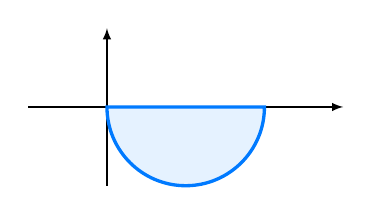
\begin{tikzpicture}
  \draw[-latex] (-1,0) -- (3,0);
  \draw[-latex] (0,-1) -- (0,1);

\filldraw[draw=lightblue, fill=lightblue!10, line width=1.2pt]
    (0,0) arc (180:360:1) -- cycle;
\end{tikzpicture}
\end{center}
  La integral se convierte en \[
    \int_{\pi}^{2\pi} \int_{0}^{1}1\cdot  r\dr \dth   =\int_{\pi}^{2\pi} \left[ \dfrac{r^2}{2} \right] _0^1\dth =\dfrac{1}{2}\int_{\pi}^{2\pi} 1\dth =\dfrac{1}{2}\cdot [\theta]_\pi^{2\pi}=\bboxed{ \dfrac{\pi}{2}}
  \] 

\item \lb{Calcular el volumen del cono de helado definido por el cono $x^2+y^2=4z^2$, $0\le z\le 1$, y el casquete superior de las esfera dado por $x^2+y^2+(z-1)^2=4,z\ge 1$.} 
  \begin{itemize}[label=\textbullet]
    \item Volumen del cono:

      La ecuación del cono $x^2+y^2=4z^2$ indica que el radio en cualquier $z$ es:  \[
      r=2z
      \] 
      El volumen del cono se calcula como:
      \[
      V_{\mathrm{cono}}=\int_{0}^{1} \int_{0}^{2\pi} \int_{0}^{2z}r\dr \dth \dz=\dfrac{4\pi}{3}
      \] 
      $\begin{array}{l}
        \int_{0}^{2z}r\dr =\left[ \dfrac{r^2}{2} \right]_0^{2z}=\dfrac{(2z)^2}{2}=2z^2 \\
        \int_{0}^{2\pi} 2z^2\dth =2z^2\cdot [\theta]_0^{2\pi}=4\pi z^2\\
        \int_{0}^{1}4\pi z^2\dz =4\pi \int_{0}^{1} z^2\dz = \pi\cdot \left[ \dfrac{z^3}{3} \right] _0^1   =\dfrac{\pi}{3}
      \end{array}$

    \item Volumen del casquete esférico superior:
\[
V_\text{casquete}=\int_{0}^{2} \int_{0}^{\frac{\pi}{2}}\int_{0}^{2\pi} r^2\sin\theta\:\mathrm{d}\varphi\dth \dr =\int_{0}^{2} \int_{0}^{\frac{\pi}{2} } 2\pi r^2\sin\theta\dth \dr =\int_{0}^{2} 2\pi r^2\dr =\dfrac{16\pi}{3} 
\] 
  \end{itemize}
  Entonces: \[
  V_{\text{total}}=V_{\text{cono}}+V_{\text{casquete}}=\dfrac{4\pi}{3}+\dfrac{16\pi}{3}=\bboxed{\dfrac{20}{3}}
  \] 
  \end{enumerate}
\end{document}
